In this chapter, we study existing techniques related to code generators testing as well as compilers auto-tuning techniques.
Section 3.1 provides a survey of the most used compiler auto-tuning techniques to construct the best set of optimization options. In Section 3.2, we review existing techniques for code generators testing. Section 3.3 discusses the limitations of the state of the art.
\section{Compilers auto-tuning techniques}

\subsection{Iterative compilation}
Iterative compilation or also known by optimization phase selection consists on applying software engineering techniques to produce better and more optimized programs by compiling multiple versions of each of them using different optimizations settings. After running these versions on specific hardware machines, the key objective of iterative compilation is to find the best optimizing sequence that lead to the fastest and better code machine code. 
Our work is related to iterative compilation research field.
The basic idea of iterative compilation is to explore the compiler optimization space by measuring the impact of optimizations on software performance.
Several research efforts have investigated this optimization problem using search-based techniques (SBSE) to guide the search towards relevant optimizations regrading performance, energy consumption, code size, compilation time, etc. Experimental results have been usually compared to standard compiler optimization levels.  

It has been proven that optimizations are highly dependent on target platform and input program. 
Compared to our proposal, none of the previous work has studied the impact of compiler optimizations on resource usage. In this work, we rather focus on compiler optimizations related to resource consumption, while bearing in mind the performance improvement.

\subsection{Implementation of iterative compilation system}
\begin{figure}[h]
	\center
	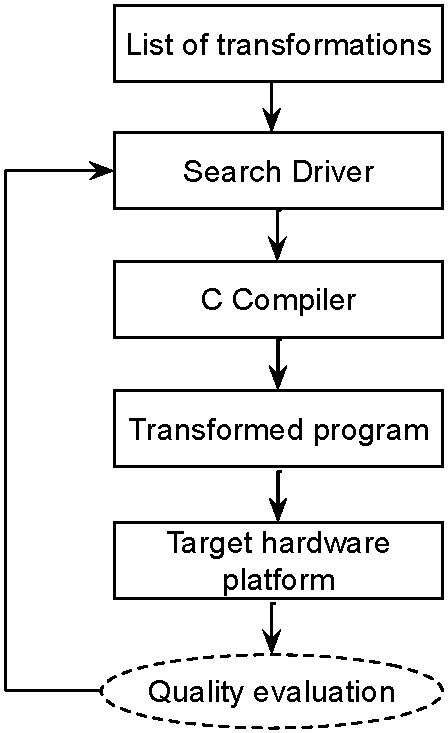
\includegraphics[scale=0.65]{SOTA/fig/iterative_compilation}
	\caption{Overview of the iterative compilation process}
	\label{fig:iterative_compilation}
\end{figure}
The implementation of iterative compilation consists mainly on applying a series of steps to enhance the quality of generated code. Figure~\ref{fig:iterative_compilation} shows a general overview of the principal steps needed to ensure the implementation of the iterative compilation process.
\begin{itemize}
	\item[--] List of transformations:
	The iterative process starts by defining the optimizations space. It represents the list of optimizations that the compiler have to apply during the search to enhance the software quality.
	\item[--] Search driver:
	It applies a search algorithm or method to efficiently explore the large optimization search space. In fact, it reads the previously defined list of transformations that it needs to examine and decides which transformations have to be applied next using a search algorithm
	to steer through the optimization space.
	\item[--] C Compiler:
	Once the optimization sequence is defined, the target C compiler for example is called to compile the input program and also perform initial machine independent optimizations. 
	\item[--] Transformed program:
	This results in initial machine independent optimized program. These optimizations are performed during code generation and have consequence for all target systems. It includes optimizations that are applied during mapping the parse tree to intermediate code and optimization applied to the intermediate code itself.
	\item[--] Target hardware platform:
	To optimize even more, the compiler applies from the provided optimization sequence the machine dependent optimizations. They are specific to the object code being generated. This includes optimizations applied during the mapping of intermediate code to assembler and optimizations applied directly on the generated
	object code.
	\item[--] Quality evaluation:
	It consists on evaluation the quality of the optimized code. Many non-functional properties could be evaluated like code size, execution time, resource usage, power consumption, etc...
	
\end{itemize}

This model represents the classical and typical iterative compilation process. Of course, there exist many ways and adaptations to implement this process. The implementation of the iterative process depends on the algorithm used, the problem addressed, the technologies used, etc. The goal of the next section is to present the different state-of-the-art approaches related to iterative compilation.

\subsection{Iterative compilation search techniques}
In section 2.5.2 of chapter 2, we presented several issues with optimizing compilers that make the activity of compiler tuning very complex such as the huge number of optimizations, conflicting objectives, optimization overhead, etc.
In this section, we discuss the available tools and approaches dedicated to the automatic search for optimal compiler settings, and give an overview of known approaches that addressed the several compiler optimization challenges. In each subsection, we identify and discuss a particular problem and we present the best known approaches proposed to solve it.

\subsubsection{Speeding up the performance: a mono objective optimization}
Speeding up the performance of compiled code is the key optimization objective for most of the iterative compilation approaches. The problem has been often adapted as a mono-objective optimization problem where the speedup has been the main concern. Genetic algorithms (GA)\cite{stephenson2003genetic,bashkansky2007black} present an attractive solution to this problem of selecting an optimal set of options. 
GA-based approaches compute an initial population using a set of optimizations, generally defined under the standard compiler levels Ox. Then, at each iteration, the individuals (i.e., option sets) that comprise the generation are evaluated by measuring for example the execution time resulted by a specific set of options. The results are sorted and pass through a breeding and mutation stage to form the next generation. This
process continues until a termination condition is reached. The algorithm return the best optimization set that led to the highest performance.

The ESTO framework described in \cite{bashkansky2007black} studies the application of GA for the problem of selecting an optimal option set for a specific application and workload. It searches the option set space using various types of genetic algorithms, ultimately determining the option set that maximizes the performance of the given application and workload. ESTO regards the compiler as a black box, specified by its external-visible optimization options. The algorithm used in ESTO is the GA. It supports also a GA variant named budget-limited genetic algorithm which reduces the population size exponentially and then reduce the time needed to evaluate the different evaluations. They ran experiments on the SPEC2000 benchmark suite and tested 60 optimization options within three compilers: GCC, XLC and FDPR-Pro. Results of ESTO are compared to GCC -O1 and -O3, to XLC -O3 and to FDPR-Pro -O3. The results show that ESTO is capable to construct optimization levels that yield to better performance than standard options.



\subsubsection{JIT compiler optimization}
\subsubsection{Escaping local optimum}
\subsubsection{Dealing with numerical parameter values}
This problem is related to numerical parameters optimization where the parameter optimization value should be determined automatically
\subsubsection{Evaluating iterative optimization across multiple data sets}
Most iterative optimization studies find the best compiler optimizations through repeated runs on input program and the same data set. The problem is that if we select the best optimization sequence for an input data set through the iterative process, we do not know if it will still be the best for the same program but with other data sets. Thereby, researchers in this field try to investigate this problem by evaluating the effectiveness of iterative optimization across a large number of data sets. In particular, since there is no existing benchmark suite with a large number of data sets  Chen et al.\cite{chen2010evaluating} attempt to collect 1000 data sets called KDataSets for 32 programs, mostly derived from the MiBench benchmark. Then, they exercise iterative optimization on these collceted data sets in order to fin the best optimization combination across all data sets. 
They used random search to generate random optimization sequences for the ICC compiler (53 flags) and the GCC compiler (132 optimizations).
They demonstrate that for all 32 programs (from MiBench), they were able to find at least one combination of compiler optimizations that achieves 86\% or more of the best possible speedup across all data sets using Intel’s ICC (83\% for GNU’s GCC). This optimal combination is program-specific and yields speedups up to 1.71 on ICC and 2.23 on GCC over the highest optimization level (-fast and -O3, respectively). This means that a program can be optimized on a collection of data sets and it can retain near optimal performance for most other data sets. So the problem of finding the best optimization for a particular program may be significantly less complex. However, they tested their approach on only one single benchmark and one target architecture.
\subsubsection{Phase ordering problem}
Phase ordering is also an important problem in iterative compilation which explores the effect of different orderings of optimization phases on program performance. In fact, using some compilers such as LLVM, it is important to define the right order of applying optimizations. Thus, researchers in this field try to apply search techniques in order to find the right optimization sequence. However, reordering optimization phases is extremely hard to support in most production systems, including GCC due to their use of multiple intermediate formats and complex inherent dependencies between optimizations. So generally, compilers manage internally the order of applying optimizations and do not give the hand to the user to choose this order to avoid conflicts and compilation issues.


\subsubsection{Conflicting objectives: a multi-objective optimization}
The vast majority of the work on iterative compilation focuses on increasing the speedup of new optimized code compared to standard compiler optimization levels. However, they do not put too much emphasis on finding trade-offs between two (or more) non-functional properties ~\cite{almagor2004finding,hoste2008cole,pan2006fast,pallister2015identifying,chen2012deconstructing,martins2014exploration,lin2008automatic,martinez2014multi}.

In COLE\cite{hoste2008cole}, the authors considered that the problem of compiler optimizations can be seen as a multi-objective problem where two non-functional properties can be enhanced simultaneously. Thus, they investigated the standard levels of compiler optimization by searching for Pareto optimal levels that maximize both performance and compile time. 
They show that by using the multi-objective genetic algorithm (in their experiment they used SPEA2), it’s possible to find a set of compiler optimization sequences that are more Pareto-effective in terms of performance and compile time than the standard optimization levels (-O1, -O2, -O3, and -Os). The motivation behind this approach is that these standard level were set up manually by compiler creators based on fixed benchmarks and data sets. For authors, these universal levels may not be always effective on unseen programs and there exist higher levels that provide better trade offs in terms of code quality.
The authors used SPEC2000 CPU benchmark, which is a popular benchmark suite for evaluating the compiler performance. They evolved 60 optimization flags that are defined in the standard levels O1, O2, O3, O1 and OS. They run iterative compilation on one single machine shipped with Intel CPU Pentium 4 and they compared the proposed algorithm (SPEA2) to random search as well as to standard optimization levels.

The experimental results using GCC (v4.1.2) show that the automatic construction
of optimization levels is feasible in practice, and in addition, yields better optimization levels than GCC’s manually derived (-Os, -O1, -O2 and -O3) optimization levels, as well as the optimization levels obtained through random sampling.
However, They do not provide a guarantee that the new explored optimization levels selected for SPEC still will be optimal for other applications.


In another story, Martinez et al.\cite{martinez2014multi} propose an adaptive worst-case execution time WCET-aware compiler framework for automatic search of compiler optimization sequences which yield highly optimized code. 
Compared to previously described approach authors in this paper focus on generating efficient code for embedded systems. Embedded systems are characterized by both efficiency requirements and critical timing constraints. Properties as Average-case performance, power consumption and resource utilization are the main concerns describing the efficiency of a system. 
Thus, they explore the performance of compiler optimizations with conflicting goals. 
Besides the objective functions average-case execution time and code size, they consider the WCET which is a crucial parameter for real-time systems, especially for
safety-critical application domains such as automotive and
avionics to avoid system failure. 
Then, they try to find suitable trade-offs between these objectives in order to identify Pareto optimal solutions using stochastic evolutionary multi-objective algorithms. The objective functions try to minimize the WCET-ACET and WCET-Code size properties. They apply three evolutionary multi-objective algorithms (EMO) namely IBEA, NSGA-II and SPEA2 and compared their results to standard levels (O1, O2 and O3). 
They evolved 30 optimizations within the WCC compiler and performed experiments on top of one single machine shipped with Intel Quad-Core CPU processor. They pick up as well 35  programs from various benchmarks such as DSPstone, MediaBench, MiBench, etc.
They found that NSGA-II is the most promising EMO for the given problem. In fact, the discovered optimization sequences significantly outperform standard optimization levels:
the highest standard optimization level O3 can be outperformed for the WCET and ACET on average by up to 31.33\% and 27.43\%, respectively. The same approach performs as well for the WCET-Code size optimization with a 30.6\% WCET reduction over O3. However, the code size increases by 133.4\%. This is because the WCET and the code size are typical conflicting goals. If a high improvement of one objective function is desired, a significant degradation of the other objective must be accepted.

\subsubsection{Predicting optimizations: a machine learning optimization}
Machine learning has been also proposed by several works to tune optimizations across programs. Compared to evolutionary algorithms, using machine learning in compiler optimization has the potential of reusing knowledge across the different iterative compilation runs, gaining the benefits of iterative compilation to learn the best optimizations across multiple programs and architectures.
In the Milepost project\cite{fursin2011milepost} for example, authors start from the observation that similar programs may exhibit similar behavior and require similar optimizations so it is possible to correlate program features and optimizations together to predict good transformations for unseen programs based on previous optimization experience. Thereby, they provide a modular, extensible, self-tuning optimization infrastructure that can automatically learn how to best optimize programs for configurable heterogeneous processors based on the correlation between program features, run-time behavior and optimizations. 

The proposed infrastructure is based on a machine learning compiler that present an Interactive Compilation Interface (ICI) and plugins to extract program features (such as the number of instructions in a method, number of branches, etc) and select optimization passes. 

The Milepost framework currently proceeds in two distinct phases: training and deployment. During the training phase, information about the structure of programs (input training programs) is gathered, showing how they behave under different optimization settings. Such information allows machine learning tools to correlate aspects of program structure, or features, with optimizations, building a strategy that predicts good combinations of optimizations. 
After running an iterative process that evaluates different combinations of optimizations on top of the training programs/features, pedictive models are created to correlate a given set of program features with profitable program transformations. 
Then, in the deployment phase, the framework analyzes new unseen programs by determining the program’s features and passes them to the new created models to predict the most profitable optimizations to improve execution time or other metrics depending on the user’s optimization requirements.

GCC was selected as the compiler infrastructure for Milepost as it is currently the most stable and robust open-source compiler. They evolved 100 optimization flags under O1, O2 and O3 levels and compared their results to the O3 level and to the random search.

The experimental results show that it is possible to improve the performance of the MiBench benchmark suite automatically using iterative compilation and machine learning on several platforms including x86: Intel and AMD, and the ARC configurable core family. Using the machine learning-based framework , they were also able to learn a model that automatically improves the execution time of some individual MiBench programs by a factor of more than 2 while improving the overall MiBench suite by 11\% on reconfigurable ARC architecture, without sacrificing code size or compilation time. Furthermore, their approach supports general multi-objective optimization where a user can choose to minimize not only execution time but also code size and compilation time.




 

\iffalse
Novelty Search has never been applied in the field of iterative compilation. Our work presents the first attempt to introduce diversity in the compiler optimization problem. 
The idea of NS has been introduced by Lehman et al.~\cite{lehman2008exploiting}. It has been often evaluated in deceptive tasks and especially applied to evolutionary robotics~\cite{risi2010evolving,krvcah2012solving} (in the context of neuroevolution). 
NS can be easily adapted to different research fields. In a previous work~\cite{boussaa2015novelty}, we have adapted the general idea of NS to the test data generation problem where novelty score was calculated as the Manhattan distance between the different vectors representing the test data. The evaluation metric of generated test suites is the structural coverage of code.
In this paper, the evaluation metric represents the non-functional improvements and we are calculating the novelty score as the symmetric difference between optimization sequences. 

For multi-objective optimizations, we are not the first to address this problem. New approaches have emerged recently to find trade-offs between non-functional properties~\cite{hoste2008cole,martinez2014multi,lokuciejewski2010multi}. Hoste et al.~\cite{hoste2008cole}, which is the most related work to our proposal, propose COLE, an automated tool for optimization generation using a multi-objective approach namely SPEA2. In their work, they try to find Pareto optimal optimization levels that present a trade-off between execution and compilation time of generated code. Their experimental results show that the obtained optimization sequences perform better than standard GCC optimization levels. NOTICE provides also a fully automated approach to extract non-functional properties. However, NOTICE differs from COLE because first, our proposed container-based infrastructure is more generic and can be adapted to other case studies (i.e., compilers, code generators, etc.). Second, we provide facilities to compiler users to extract resource usage metrics using our monitoring components. Finally, our empirical study investigates different trade-offs compared to previous work in iterative compilation.
\fi





%For code generators testing, Stuermer et al.~\cite{stuermer2007systematic} present a systematic test approach for model-based code generators. They investigate the impact of optimization rules for model-based code generation by comparing the output of the code execution with the output of the model execution. 
%If these outputs are equivalent, it is assumed that the code generator works as expected. 
%They evaluate the effectiveness of this approach by means of testing optimizations performed by the TargetLink code generator. 
%They have used Simulink as a simulation environment of models. 
%In our approach, we provide a component-based infrastructure to compare non-functional properties of generated code rather than functional ones. 


\section{Testing code generators}
Previous work on non-functional testing of code generators focuses on comparing, as oracle, the non-functional properties of hand-written code to automatically generated code~\cite{stepasyuk2015evaluating,richard2013efficient}. As an example, Strekelj et al.~\cite{vstrekelj2015performance} implemented a simple 2D game in both the Haxe programming language and the native environment and evaluated the difference in performance between the two versions of code. They showed that the generated code through Haxe has better performance than hand-written code. 

Cross-platform mobile development has been also part of the non-functional testing goals since many code generators are increasingly used in industry for automatic cross-platform development. In \cite{pazirandeh2015evaluation,hartmann2011cross}, authors compare the performance of a set of cross-platform code generators and presented the most efficient tools.

The container-based infrastructure has been also applied to the software testing, especially in the cloud~\cite{li2015rest}. Sun et al.~\cite{sun2016roar} present a tool to test, optimize, and automate cloud resource allocation decisions to meet QoS goals for web applications. Their infrastructure relies on Docker to gather informations about the resource usage of deployed web servers. 

Most of the previous work on code generators testing focuses on checking the correct functional behavior of generated code. Stuermer et al.~\cite{stuermer2007systematic} present a systematic test approach for model-based code generators. They investigate the impact of optimization rules for model-based code generation by comparing the output of the code execution with the output of the model execution. 
If these outputs are equivalent, it is assumed that the code generator works as expected. 
They evaluate the effectiveness of this approach by means of testing optimizations performed by the TargetLink code generator. 
They have used Simulink as a simulation environment of models. 
In \cite{jorges2014back}, authors presented a testing approach of the Genesys code generator framework which tests the translation performed by a code generator from a semantic perspective rather than just checking for syntactic correctness of the generation result.

Compared to our proposal, none of the previous work has provided an automatic approach for testing and monitoring the generated code in terms of non-functional properties. 





\subsection{The oracle problem}
Most of the work on software testing seeks to automate as much as possible the testing process to make it faster, cheaper, and more reliable. 

To this end, automatic program testing involves in selecting suitable inputs as test cases, executing the program and verifying results against expected results. 
The mechanism against which the software tester verify whether the outputs of the program for the executed test cases are correct or not is called \textit{test oracle}. 

For instance, the problem of automatically generating test inputs/data has been the subject of research interest for a long time. It consists on automatically generating test data/cases in order to detect faults/crashes or to maximize the code coverage of the program under test. 


Research in software testing has focused on automating many aspects of the testing process such as test data generation, test cases generation and execution, test suites reduction, test cases prioritization, etc. Many techniques especially search-based testing techniques have been proposed to solve and automate these processes\cite{ali2010systematic}.

However, compared to many aspects of test automation, the problem of automating the test oracle is still challenging and less well solved. Only few techniques are available to generate test oracles. In most of the cases designing and implementing test oracles are still manual and expensive activities. That is because the test oracles are not always available and may be hard to define or too difficult to apply\cite{barr2015oracle}. This is commonly known as the \textit{"oracle problem"}. 

As pointed out in\cite{manolache2001software}, the oracle problem has been “one of the most difficult tasks in software testing” but it is often ignored by researchers in software testing.

For example, let \textit{sine} be a function implementing a specification \textit{S}. Let \textit{D} represent the input domain which represents the input values for which we would calculate the \textit{sine}. Usually, the testing process should verify if the \textit{sine(x) = S(x)} $\forall$ \textit{x} $\in$ \textit{D}. The procedure through which the testing program can check whether \textit{sine(x) = S(x)} is called an oracle.

Automatically generating  \textit{D} (test data) and executing test cases in this example is simple. It consists on generating random numerical values for example. However, it is impossible to do an exhaustive testing to automatically check the expected output.

For instance, only the special input values  \textit{0}, $\pi/4$,  $\pi/2$, etc., could be the standard test cases since the output of  \textit{sine(x)} for these test data values is known and can be automatically checked against the specification. Nevertheless, special values cannot give us enough confidence in the correctness of the program on more complex or random inputs. 

Other examples include, testing programs calculating numerical functions or solving complex equations; testing programs that calculate combinatorial problems, testing graphical user interfaces, etc.

Automatically testing generators also implies the oracle problem. When testing compilers for example, it is quite difficult to automatically verify the equivalence between the source code and object code. This task becomes even more complicated when some optimizations are applied to the machine code. 

When testing code generators, the verification of the high level system specification with the generated code is also challenging. Supposing that the \textit{sine} function is defined using a high level language. The generated \textit{sine} function should be evaluated with the same effort as the manual written code in order to verify whether the code generator has introduced bugs or not. 

%SINE + MEtamorphic testing
%When testing a program p supposedly implementing the sine function, for example, let 1.28 be a test case. Although we do not know the exact value of sin1.28, a failure can still be identified if the output p(1.28) > 1 because |sinx| ≤ 1 ∀x ∈ R. By employing more mathematical properties of the sine curve, the range of plausible values of p(1.28) can be further narrowed down greatly.



The research community has proposed several approaches to alleviate the oracle problem. 
Stocks and Carrington discuss an approach for deriving test cases and oracles from specification.
Test oracles can be associated with individual test templates (test case specifications). A hierarchical arrangement of test templates allows the oracle to
be either general (near the top of the hierarchy) or specialized to particular test cases.
The approach is illustrated with test oracle templates for the Z specification in Example
23


Richardson et al. [5] propose an approach to deriving and using specification-based oracles in the
testing process. Peters and Parnas [6,7] developed a test-oracle generator that produces a software
oracle from relational program documentation. Unfortunately, formal methods have not been widely
adopted in industry yet. A major obstacle seems to be the lack of compelling evidence of their
effectiveness for industrial-size applications [9]. Specification-based oracles might be the answer for
the future, but in the meantime the industry needs better approaches to the oracle problem than manual
outcome prediction. Both Weyuker [10] and Beizer [4] suggest several practical alternatives. One
of them is to build a pseudo-oracle in the form of a detailed prototype or a dual program that is
capable of providing the expected outputs. The approach examined here is similar and is based on
N-version diversity, a principle that is applied especially in the well-known software fault-tolerant
technique known as N-version programming. To highlight its similarity with N-version programming,
the approach advocated below is called ‘testing using M model programs’ or, in short, ‘M-mp testing’.


\subsection{Metamorphic testing techniques}

A metamorphic testing (MT) method has been proposed to alleviate the oracle problem\cite{chen2004case}. MT is an automated testing method that employs expected properties of the target functions to test programs without human implication. 
MT recommends that, given one or more test cases (called source or original test cases) and their expected outcomes, one or more follow-up test cases can be constructed to verify the necessary properties (called Metamorphic Relations MRs) of the system or function to be implemented.
For a given problem, usually more than one MR can be identified. It is therefore interesting to select effective MRs that are good at detecting program bugs.



\section{Container-based testing techniques}

Using virtual machines (VMs) as a mechanism for deploying and testing applications in the cloud is very useful to run applications workload in heterogeneous and distributed environments.
In industry, a number of commercial usage scenarios benefit from virtualization techniques to provide services to the end users. For example, Amazon EC2 makes VMs available to the customers who can use them to run their own computer applications or services on the cloud. Thus, a user can create, launch and terminate new VMs as needed.  

However, VMs are known to be very expensive in terms of system resources and performance. In fact, each new VM instance constitutes of a virtual copy of all the hardware of the host machine which adds a lot of resource usage and overhead\cite{merkel2014docker}. 

Container-based virtualization presents an interesting alternative virtualization technology to virtual machines in the cloud. Containers is an operating-system-level virtualization which imposes little to near zero overhead. Programs in virtual instances use the operating system's system call interface and do not need to be emulated or run in an intermediate virtual machine, as is the case VMs such as VMware, QEMU or Xen.
Docker offers the ability to deploy applications and their dependencies into lightweight containers that are very cheap to create and isolated form each other. Processes executing in a Docker container are isolated from processes running on the host OS or in other Docker containers. The Docker solution aims to address the challenges of resource, speed and performance of virtualization in the software development process. 

Authors of \cite{spoiala2016performance,soltesz2007container,merkel2014docker,felter2015updated} used to compare the performance of traditional virtual machine solution that isolate VMs at the hardware abstraction layer to container-based operating system technology that isolate VMs at the system call layer. They showed that containers result in better performance than VMs since thay induce less overhead. 

\subsection{Deployment and testing using Docker}  
In software development, the container technology becomes more and more used in order to create a portable, consistent operating environment for development, deployment and testing.

In the following, we will focus and discuss state of the art approaches that chose the container technology as an efficient infrastructure to solve some testing research problems. 


Marinescu et al.\cite{marinescu2014covrig} have used Docker as technological basis in their repository analysis framework Covrig to conduct a large-scale and yet safe inspection of the revision history from six selected Git code repositories. 
For their analysis, they used to run each version of a system in isolation and collect static and dynamic software metrics, using a lightweight container environment that can be deployed on a cluster of local or cloud machines. Each container is used to configure, compile and test one program revision, as well as collect the metrics of interest, such as code size and coverage.
The motivation of using such infrastructure is to provide a clean and configurable execution environment to run experiments. According to the authors, the use of Docker as a solution to automatically deploy and execute the different program reversions and test suites has clearly facilitated the testing process.


Another Docker-based approach is presented in the BenchFlow2 project which focuses on benchmarking BPMN 2.0 engines\cite{ferme2015framework}. This project is dedicated to the performance testing of workflow engines. In this work, Ferme et al present a framework for automatic and reliable calculation of performance metrics for BPMN 2.0 WfMSs. 

According to the authors benchmarking WfMSs raises many challenges: 1) the system deployment complexity due to the distributed nature of these models execution; 2) the high number of configuration options require to integrate the configuration and the deployment of the SUT, i.e., the WfMS, as part of the performance test definition; 3) the complexity of the execution behaviours that can be expressed by modern modeling and execution languages such as BPMN2.

Therefore, to address these problems, BenchFlow exploits \textbf{Docker} as a containerization technology, to enable the automatic deployment and configuration of the WfMS and to ensure that the experimental results can be reproduced.
Thus, the WfMSs are automatically deployed and undeployed using Docker. Each component involved in the benchmark are packaged as Docker images
to be deployed and executed on different servers connected by a dedicated local
network. For each Docker instance, a new instance of the BP models set is executed by the WfE during the experiment.

Thanks to Docker, BenchFlow automatically collects all the data needed to compute performance metrics, and to check the correct execution of the tests (metrics related the RAM/CPU usage and execution time).
Their experimental results show that a simple BP model running on two popular
open-source WfMSs have uncovered important performance scalability issues. 

Hamdy et al.\cite{hamdy2016web} propose Pons, a web based tool for the distribution of pre-release mobile
applications for the purpose of manual testing. Pons facilities building, running, and manually testing of Android applications directly in the browser. 
Based on Docker technology, this tool gets the developers and end users engaged in testing the applications in one
place, alleviates the tester's burden of installing and maintaining testing environments, and provides a platform for developers to rapidly iterate on the software and integrate changes over time. Thus, it speeds up the testing process and reduces its cost.

Pons utilizes Docker by predefining Docker images that
contain the necessary services and tools to build android
applications, starting from the operating system up to the
software development kit (SDK). A container is then built using one of these images to store the source code of
a mobile application at specific moment of history in a
sandbox environment. Pons creates then, an android emulator inside the docker container to run the tests. The results are streamed at runtime in the web browser.

\subsection{Runtime monitoring using Docker} 

 

Runtime monitoring is an essential part of cloud computing\cite{aceto2013cloud}. Like virtual machines before them, containers require a monitoring mechanism. It should provide both historical and timely information about the resource usage from hardware to virtual machine and container level.


To have a true perspective on the performance for containerized environments, container users have to monitor both the host and the containers. There are multiple options for monitoring. 
Among the popular ways to do that is to monitor each container via the Docker API, or by installing an agent inside each container for detailed visibility inside each container. 

The Docker client for example already provides a command line tool to inspect containers’ resource consumption. The command \textit{docker stats} for example,can be used to get stats about the running containers at runtime. This will present the CPU utilization for each container, the memory used and total memory available to the container.

Linux Containers rely on cgroups (control groups) which is a Linux kernel feature that limits, accounts for, and isolates the resource usage (CPU, memory, disk I/O, network, etc.) of a collection of processes.
Cgourps do not only track groups of processes, but also expose metrics about CPU, memory, and block I/O usage. 

In industry, many commercial solutions are proposed to offer facilities to container users to efficiently monitor their workload inside containers. Most of these solutions rely on automatic cgroups metrics extraction and provide a visual representation of the data shown by the docker stats command. For example, the Datadog\footnote{www.datadoghq.com} and cAdvisor\footnote{https://github.com/google/cadvisor} agent uses the native cgroup accounting metrics to gather CPU, memory, network and I/O metrics of the containers. CAdvisor allows to monitor containers that run in the same host machine. However, Scout\footnote{https://scoutapp.com} is a hosted monitoring service which can aggregate metrics from many hosts and containers and present the data over longer time-scales. It can also create alerts based on those metrics. 

Most of these tools provide web-based dashboards to visualize resource consumption at runtime as well as alerting mechanism to that can be triggered if metrics go above or below a configured threshold. Other examples of monitoring docker tools: Sensu Monitoring Framework, Prometheus, Sysdig Cloud, etc.
Tools like cAdvisor and Prometheus allow to monitor containers running on one single host machine. 

However, there are many applications to manage the execution of containers across multiple hosts. For example, Kubernetes\footnote{https://kubernetes.io} is an open source orchestration system for Docker containers. It allows to quickly and efficiently respond to customer demand by deploying applications using multiple hosts and containers on the cloud, scale applications on the fly and optimize the resource usage across multiple hosts. This clustering framework is shipped with a monitoring tool called Hipster\footnote{https://github.com/kubernetes/heapster} that provides a base monitoring platform on Kubernetes. Heapster collects and interprets various signals like resource usage, lifecycle events, etc, and exports cluster metrics via REST endpoints. It supports a pluggable storage backend such as InfluxDB with Grafana and Google Cloud Monitoring.


In the research filed, \cite{kookarinrat2015analysis} Kookarinrat et al. have investigated the problem of auto-sharding in No-sql databases using a container-based infrastructure for runtime monitoring. 
The auto-sharding technique is used to divide data in the database and distribute it over multiple machines in order to scale it horizontally. The motivation behind this work is that selecting a right key is challenging. It could lead to either an improve of the performance and capability of a database or to performance issues (i.e., by selecting a wrong key) which could lead to a system halt. 
For instance, a good shard key should have high degree randomness for write scaling and should contain high locality for range-query reading.
Therefore, they analyzed and evaluated such suggested properties by studying how the variation of a shard key’s choices could impact the DB performance.

They simulated an environment using Docker containers and measured the read/write performance of variety of keys. Inside each container, they executed write/read queries into the MongoDB database and used docker stats to retrieve automatically information about the memory and CPU usage of inside each container.

They found that a shard key with randomness and good locality could give a decent performance on write and
read. However, in case that a shard key has nearly sorted values, combining a small range of random values to it might give acceptable performance for both read and write. 
 

Container monitoring tools discussed above have been used in several other works like in\cite{peinl2016docker,medel2016modelling}.
\section{Summary}
 



\iffalse
Our work is related to iterative compilation research field.
The basic idea of iterative compilation is to explore the compiler optimization space by measuring the impact of optimizations on software performance.
Several research efforts have investigated this optimization problem to catch relevant optimizations regrading performance, energy or code size improvements over standard optimization sequences~\cite{almagor2004finding,hoste2008cole,pan2006fast,zhong2009tuning,pallister2015identifying,chen2012deconstructing,sandran2012genetic,martins2014exploration,fursin2008milepost,lin2008automatic,schulte2014post}. 
The vast majority of the work on iterative compilation focuses on increasing the speedup of new optimized code compared to standard optimizations. 
It has been proven that optimizations are highly dependent on target platform and input program. Compared to our proposal, we rather focus on comparing the resource consumption of optimized code.

Novelty Search has never been applied in the filed of iterative compilation. Our work presents the first attempt to introduce diversity in optimization sequences generation. The idea of NS has been introduced by Lehman et al.~\cite{lehman2008exploiting}. It has been often evaluated in deceptive tasks and especially applied to evolutionary robotics~\cite{risi2010evolving,krvcah2012solving} (in the context of neuroevolution). 
NS can easily be adapted to different research fields. In a previous work~\cite{boussaa2015novelty}, NS has been adapted for test data generation where novelty score was calculated as the Manhattan distance between the different vectors representing test data.
In our NS adaptation, we are measuring the novelty score using the systematic difference between optimization sequences of GCC.

For code generators testing, Stuermer \etal present a systematic test approach for model-based code generators~\cite{stuermer2007systematic}. They investigate the impact of optimization rules for model-based code generation by comparing the output of the code execution with the output of the model execution. 
If these outputs are equivalent, it is assumed that the code generator works as expected. 
They evaluate the effectiveness of this approach by means of testing optimizations performed by the TargetLink code generator. 
They have used Simulink as a simulation environment of models. 
In our approach, we provide a component-based infrastructure to compare non-functional properties of generated code rather than functional ones. 
\fi
